\clearpage
\section{Cosmological simulations}

In this section, we describe in more detail how RAMSES can be used to
perform cosmological simulations. Useful concepts related to parallel
computing or post-processing will be introduced, and can also be used
for non-cosmological runs. Cosmological simulations are performed by
specifying \cmd{\nmlentry{cosmo}=.true.} in the \nmlblock{\&RUN\_PARAMS}
namelist.

\subsection{Parameter file and initial conditions}
\label{sec:cosmo_init}

The first thing to do when performing cosmological simulations is to
generate initial conditions as Gaussian random fields. The easiest way
is to use the freely available \pkg{grafic2} code, developed by Edmund
Bertschinger at MIT (see \url{http://web.mit.edu/edbert}) or its
parallel version \pkg{mpgrafic} developed by Christophe Pichon and Simon
Prunet at IAP (see \url{http://www.projet-horizon.fr/}). These codes
will generate initial conditions according to a given cosmological model
and for a given box size. As outputs, 7 files will be generated, called
\cmd{ic\_deltab}, \cmd{ic\_velcx}, \cmd{ic\_velcy}, \cmd{ic\_velcz},
\cmd{ic\_velbx}, \cmd{ic\_velby} and \cmd{ic\_velbz}. The directory in
which these files are stored should be entered in the Parameter File as
parameter \cmd{\nmlentry{initfile}(1)} in namelist
\nmlblock{\&INIT\_PARAMS}. Index 1 stands here for \nmlentry{levelmin},
and corresponds to the coarse grid.  RAMSES will automatically read the
cosmological parameters and the physical box length contained in these
initial conditions files. The so-called ``super-comoving'' coordinate
system is used in RAMSES for cosmological runs (see Martell \& Shapiro
2003). \ If necessary, the translation from this scale-free coordinate
system (\cmd{\nmlentry{boxlen}=1.0}) to the \emph{cgs} system is
performed using scaling factors stored in the output files. The units
are set in routine \cmd{units.f90} in directory \dir{amr/}.

The following namelist can be found in directory \dir{namelist/} in the
RAMSES package as file \cmd{cosmo.nml}. It is the Parameter File for a
pure $N$-body simulation, using $128^3$ particles and a $128^3$ coarse
grid with 7 additional levels of refinement. To specify that initial
conditions are to be read in grafic files,
\cmd{\nmlentry{filetype}='grafic'} should be set in namelist
\nmlblock{\&INIT\_PARAMS}.

\logfile{userfiles/cosmo.nml}

Parameters \nmlentry{ngridtot} and \nmlentry{nparttot} specify the
maximum memory allocated for AMR grids and collisionless particles
respectively. These numbers should be greater than or equal to the
actual number of AMR grids and particles used during the course of the
simulation.

\nmlentry{ngridtot} stands for the total number of AMR grids allocated
over all MPI processes. The \nmlentry{ngridmax} parameter can be used
equivalently, but stands for the local number of AMR grids within each
MPI process. Obviously, one has \cmd{ngridtot=ngridmax*ncpu}.

\begin{warning}
Recall that, in RAMSES, we call ``AMR grid'' or ``oct'' a group of
$2^{\mathtt{ndim}}$ cells. If for some reason, during the course of the
execution, the maximum allowed number of grids or particles has been
reached, the simulation stops with the message:
%
\begin{Prompt}
 No more free memory
 Increase ngridmax
\end{Prompt}
%
In this case, don't panic: just increase \nmlentry{ngridmax} in the
Parameter File and resume the execution, starting from the last backup
file.
\end{warning}


\subsection{Memory management}

These two parameters control the memory allocated by RAMSES. It is
important to know how much memory in Gb is actually allocated by RAMSES
for a given choice of parameters. This can be approximated by:

\begin{itemize}
\item $0.7 (\nmlentry{ngridmax}/10^6) + 0.7 (\nmlentry{npartmax}/10^7)$
Gbytes for pure $N$-body runs,
\item $1.4 (\nmlentry{ngridmax}/10^6) + 0.7 (\nmlentry{npartmax}/10^7)$
Gb for $N$-body and hydro runs,
\item $1.0 (\nmlentry{ngridmax}/10^6)$ Gb for pure hydro runs.
\end{itemize}

Because of MPI communications overheads, the actual memory used can be
slightly higher. Note that these numbers are valid for double precision
arithmetic. For single precision runs, using the preprocessor directive
\cmd{-D\cflag{NPRE}=4}, you can decrease these figures by 40\%.
% TODO: warning about single precision here

\subsection{Restarting a run}

As we just discussed, it is possible to resume a RAMSES run if the
execution has stopped abnormally. For that, RAMSES uses its output
files, stored in directories called

\begin{Verbatim}
output_00001/
output_00002/
output_00003/
output_00004/
\end{Verbatim}

Each directory contains all the necessary information for RAMSES to
resume the execution. The frequency at which these output files are
created is specified by parameter \nmlentry{foutput}, in units of coarse
time steps. If you want to resume the execution starting from output
directory number 4, you need to specify the corresponding number in
parameter \cmd{\nmlentry{nrestart}=4}. If you set
\cmd{\nmlentry{nrestart}=0}, the run will start from the beginning as a
completely new run.

\begin{warning}
When restarting a job, you can change almost all run parameters. There
are however some notable exceptions: The number of output times can only
be increased, and only new output times can be added after the old ones.
The number of processors used with MPI cannot change. If you want to
change the number of processes, you should start from the very
beginning.
\end{warning}

\subsection{Parallel computing}

We are now ready to address the complex issue of parallel computing
with RAMSES. It is based on the MPI library through regular calls of MPI
communication routines. In order to compile and link RAMSES with the MPI
library, you need first to remove the preprocessor directive
\cmd{-D\cflag{WITHOUTMPI}} from the compilation options in the Makefile.
Don't forget to type \cmd{make clean} and then \cmd{make} again.

In order to launch a parallel RAMSES run, type for example

\begin{Prompt}
\$ mpirun -np 4 bin/ramses3d namelist/sedov3d.nml
\end{Prompt}

The two key parameters for parallel runs are \nmlentry{nremap} and
\nmlentry{ordering}, both contained in the \nmlblock{\&RUN\_PARAMS}
namelist block. The first one specifies the frequency at which the code
will optimize load balancing by adjusting the domain decomposition, in
units of coarse time step. Since it is a rather costly operation, this
should not be performed too frequently. On the other hand, if the AMR
grid evolves significantly with time, the computational and memory load
might be very inhomogeneous across the processors. The optimal choice
for parameter \nmlentry{nremap} is therefore application-dependent. Bear
in mind that if \cmd{nremap>10}, the associated overhead should be
negligible.

The other important parameter for an efficient parallel computing
strategy is \nmlentry{ordering}. This character string specifies the type
of domain decomposition you want to use. There are 3 possible choices in
RAMSES currently implemented: \cmd{'hilbert'} (default value),
\cmd{'planar'} and \cmd{'angular'}. Each cell in RAMSES is ordered with
an integer index according to a given space ordering. One of the most
famous ordering used in computer science is the Peano-Hilbert
space-filling curve. This is a one-dimensional object filling up the
three-dimensional space. An example of such domain decomposition is
shown in figure \ref{fig:hilbert}. This strategy is known to be the
optimal choice if one considers the rather large ensemble of all
possible AMR grids. In some cases, however, it is no longer an
efficient strategy. The planar decomposition, for example, sets up
computational domains according to one coordinate only (the altitude $z$
for example). Each processor receives a layer of cells whose thickness
is automatically adjusted in order to optimize load balance. The angular
decomposition follows the same strategy, except that now the coordinate
is the polar angle around a given axis in the simulation box. These
various orderings can be adapted easily to account for specific
constraints. The user is encouraged to edit and modify the routine
\cmd{load\_balance.f90} in directory \dir{amr/}.

\begin{figure}
   \begin{center}
   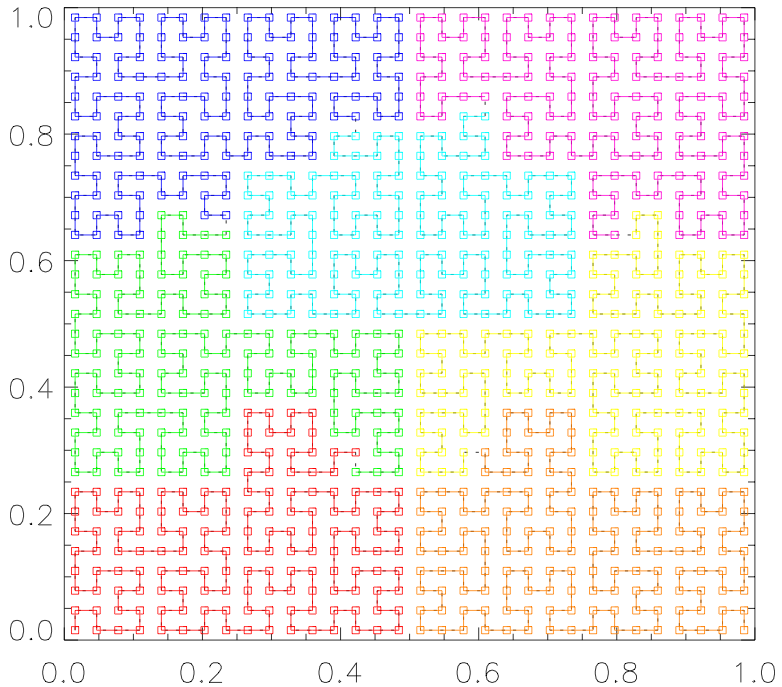
\includegraphics[width=0.8\textwidth]{img/hilbert.png}
   \end{center}
   \caption{Domain decomposition of the unit square for a $32^2$ grid
   over 7 processors using the Peano-Hilbert space-filling curve
   shown as the continuous line.}
   \label{fig:hilbert}
\end{figure}


In case of parallel execution, RAMSES performs hard disk outputs in a very
simple way: each processor creates its own file. Therefore, in directory
\dir{output\_00001/}, one can find several files with a numbering
corresponding to the processor number. One should bear this in mind when
using the snapshots generated by RAMSES.

\subsection{Post-processing utilities}

Several post-processing codes are available in the current package in
directory \dir{utils/f90}. These are very simple pieces of software
performing rather basic operations on RAMSES generated outputs. Users are
encouraged to edit and modify these routines in order to design specific
post-processing applications. We briefly describe them now.

\begin{itemize}
\item \util{amr2map}: this application reads RAMSES outputs and
generates a projected map along one principal axis. The output is a
binary Fortran image that can be read using any image-processing tool.
\item \util{amr2cube}: this application reads RAMSES outputs and
generates a 3D Cartesian cube with only one flow variable represented.
The output is a binary Fortran file (raw data or grafic data) or a VTK
file that can be read using any data visualization tool.
\item \util{part2map}: this application reads RAMSES outputs for
collisionless particles only and projected the particle distribution
along one principal axis. The output is a binary Fortran image.
\item \util{part2cube}: this application reads RAMSES outputs for
particles only and generates a CIC interpolated density field. The
output is a binary Fortran file.
\end{itemize}

Each one of these codes is a stand-alone application that can be
compiled straightforwardly by typing directly for example:

\begin{Prompt}
\$ f90 amr2map.f90 -o amr2map
\end{Prompt}

In directory \dir{utils/idl}, you can find a set of IDL routines to be
used in order to display AMR data using IDL (see
\url{http://www.ittvis.com/}).  Here is an example of interactive
commands you need to type within your IDL session to watch RAMSES data
(for example using \cmd{sedov2d.nml}).

\begin{Prompt}
IDL> rd_amr,a,nout=2   ; Read AMR data from snapshot nr 2 and store in a
IDL> rd_hydro,h,nout=2 ; Read hydro data and store in variable h
IDL> window,0,xs=512,ys=512       ; Set up a square window
IDL> loadct,33                    ; Load a nice color table
IDL> tv2d,a,h,type=1,/log,/show   ; Plot a density map with the grid
\end{Prompt}
%
Here is another example to plot a density profile from the previous
data.
%
\begin{Prompt}
IDL> amr2cell,a,h,c        ; Convert AMR data into cell-based data
IDL> r=sqrt(c.x^2+c.y^2)   ; Compute cell radius
IDL> d=c.var(*,0)          ; Compute cell density
IDL> plot,r,d,psym=6
\end{Prompt}
%
For 3D data, you can use a simple raytracing algorithm to project
various quantities along one of the box principal axis.
%
\begin{Prompt}
IDL> ray3d,a,h,lmin=7,lmax=9,/zproj,/ave,type=1,/log
          ; Project the average density along the z-axis
\end{Prompt}


\subsection{Zoom simulations}

Another interesting cosmological application for RAMSES is the so-called
``zoom'' technology or ``re-simulation'' process. Let us consider the
large-scale periodic box simulation we have presented in the previous
section, performed with $128^3$ particles by RAMSES with the
\pkg{grafic} files stored in directory \cmd{/scratchdir/grafic\_files}.
After using the \util{sod} application, all dark matter halos in the
final output have been identified. One halo is believed to be a good
candidate for re-simulation. A quasi-spherical region must be
determined, whose size and position are optimized in order to contain
all the particles ending up in the final halo. A new set of initial
conditions must then be generated using \pkg{mpgrafic}, providing the
same large-scale modes than the previous run, but allowing now to
simulate up to $1024^3$ particles.
A suite of applications is available in directory \dir{utils/f90} to
perform the extraction of a high-resolution region containing the halo
particles only. These codes are called \util{center\_grafic},
\util{extract\_grafic} and \util{degrade\_grafic}. The idea is to center
the simulation box on the high-resolution region, to extract a nested
collection of rectangular grids around this position with various
particle masses.  The initial conditions data for each box are stored in
a different directory. The original data centered on the region center
can be called \cmd{boxlen100\_n256}, where \cmd{100} stands for the box
size in $h^{-1}$ Mpc and \cmd{128} for the number of particles per box
length. The nested box hierarchy we obtained using our various utilities
is now:
%
\begin{Verbatim}
boxlen100_n128/
boxlen50_n128/
boxlen25_n128/
boxlen12p5_n128/
\end{Verbatim}
%
Each of these directories should contain 7 grafic files. These names
should be now inserted in the Parameter File, in the
\nmlblock{\&INIT\_PARAMS} block, as
%
\begin{Verbatim}
&INIT_PARAMS
filetype='grafic'
initfile(1)='/scratchdir/grafic_directories/boxlen100_n128'
initfile(2)='/scratchdir/grafic_directories/boxlen50_n128'
initfile(3)='/scratchdir/grafic_directories/boxlen25_n128'
initfile(4)='/scratchdir/grafic_directories/boxlen12p5_n128'
/
\end{Verbatim}
%
The re-simulation is now ready to go. Those are our last words on
cosmological simulations and how to run them using only Parameter Files
as Runtime Parameters. We now describe how to use RAMSES with more
advanced settings.
